\documentclass{article} % For LaTeX2e
\usepackage{nips13submit_e,times}
\usepackage{hyperref}
\usepackage{url}
\usepackage{graphicx}
\graphicspath{ {images/} }
%\documentstyle[nips13submit_09,times,art10]{article} % For LaTeX 2.09


\title{Clustering Wikipedia Articles}


\author{
Lane Aasen\\
Department of Computer Science\\
University of Washington\\
Seattle, WA 98105\\
\texttt{aaasen@cs.washington.edu}\\
}

% The \author macro works with any number of authors. There are two commands
% used to separate the names and addresses of multiple authors: \And and \AND.
%
% Using \And between authors leaves it to \LaTeX{} to determine where to break
% the lines. Using \AND forces a linebreak at that point. So, if \LaTeX{}
% puts 3 of 4 authors names on the first line, and the last on the second
% line, try using \AND instead of \And before the third author name.

\newcommand{\fix}{\marginpar{FIX}}
\newcommand{\new}{\marginpar{NEW}}

\nipsfinalcopy % Uncomment for camera-ready version

\begin{document}


\maketitle

\begin{abstract}
Clustering Wikipedia articles using unsupervised learning techniques including K-Means, Latent Dirichlet Allocation (LDA), and spectral clustering.
\end{abstract}


\section{Dataset}

The provided dataset contains 15,903 Wikipedia articles in tf-idf format. There are 10,574 unique words in this dataset. Each document is represented as a sparse vector with one dimension for each word. I have not experimented with dimensionality reduction yet, but it could be an interesting topic to explore.

\section{K-Means Clustering}

For the project milestone, I have implemented K-Means clustering on the provided subset of Wikipedia articles.

\subsection{Choosing K}

\subsubsection{Minimizing Distortion}

Given $K$ clusters $C_{1},C_{2},...,C_{K}$ where each cluster is a set of document vectors and $\mu_{i}$ is the centroid of $C_{i}$, the total distortion is defined as follows:

$$\sum_{i=1}^{K}\sum_{d \in C_{i}} ||d - \mu_{i}||^{2}$$

To minimize the distortion, we could set $K$ equal to the number of documents, but then the clusters would be meaningless. We want to choose a K with low distortion that also results in interpretable clusters. Figure 1 shows a plot of K versus total distortion. When $1 \leq K \leq 16$, adding additional clusters has a large impact on the distortion. However, once $K > 16$, adding additional clusters has little impact on the distortion. From this alone, it makes sense to set $K=16$ since it provides a good balance of distortion and interpretability.


\begin{figure}[h]
\begin{center}
\framebox{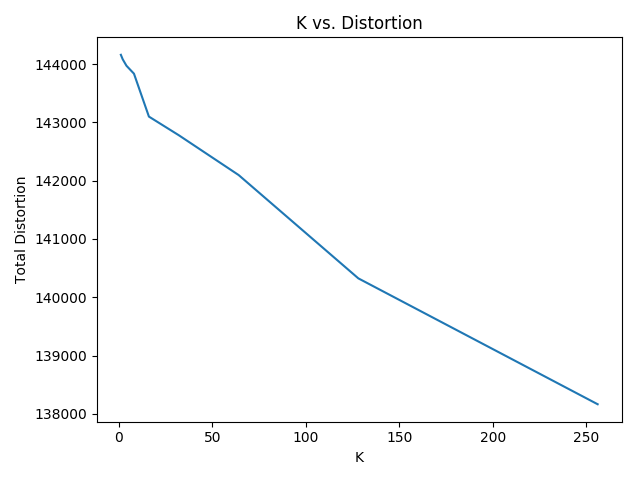
\includegraphics[scale=0.5]{k_vs_distortion}}
\end{center}
\caption{$K$ versus total distortion for $K \in \{1,2,4,...,256\}$}
\end{figure}

\subsection{K and Cluster Size}

As $K$ increases, the clusters become more sparse. Once $K=256$, over half of the clusters have only one document, and are essentially useless. When $K=16$, the median cluster size is 8.5, and the cluster sizes are as follows:

$$[10061, 3013, 1128, 909, 707, 30, 23, 13, 4, 4, 3, 2, 2, 2, 1, 1]$$

Over half of the clusters are very small, and one of the clusters is too large to be interpretable. This indicates that the data has significant outliers and lacks a structure conducive to clustering.








In a perfect dataset with $n$ documents and $K$ clusters, we would expect each cluster to have exactly $K/n$ documents.

\begin{figure}[h]
\begin{center}
\framebox{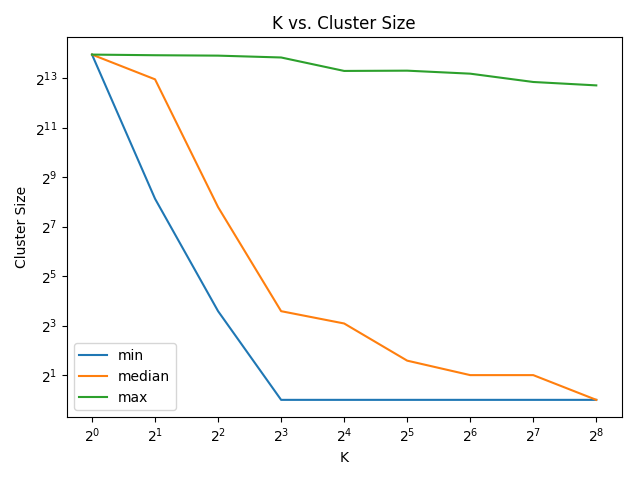
\includegraphics[scale=0.5]{k_vs_cluster_size}}
\end{center}
\caption{$K$ versus minimum, median, and maximum cluster size for $K \in \{1,2,4,...,256\}$ with a $log_{2}$ scale on both axes.}
\end{figure}

\subsection{Tables}

All tables must be centered, neat, clean and legible. Do not use hand-drawn
tables. The table number and title always appear before the table. See
Table~\ref{sample-table}.

Place one line space before the table title, one line space after the table
title, and one line space after the table. The table title must be lower case
(except for first word and proper nouns); tables are numbered consecutively.

\begin{table}[t]
\caption{Sample table title}
\label{sample-table}
\begin{center}
\begin{tabular}{ll}
\multicolumn{1}{c}{\bf CLUSTER}  &\multicolumn{1}{c}{\bf SIZE}
\\ \hline \\

\end{tabular}
\end{center}
\end{table}


\end{document}
